\documentclass{article}
\usepackage[export]{adjustbox}
\usepackage{url}
\usepackage[top=2cm, bottom=2cm, outer=2cm, inner=2cm]{geometry}
\begin{document}
\begin{center}
\vspace*{8cm}
\textsf{\begin{Huge}
\textbf{Computer Networks \\[5pt]
NPTEL Notes}
\end{Huge} }
\end{center}
\pagebreak
\tableofcontents
\pagebreak
\section{Formal Framework - Protocols}
\begin{enumerate}
\item Building blocks of a network architecture.
\item Each protocol object has two interfaces.
\begin{enumerate}
\item \textit{Service interface} defines the operations of the protocol.
\item \textit{Peer to peer interface} defines messages exchanged with peer.
\end{enumerate}
\end{enumerate}
\vspace{5cm}
\section{Protocol Hierarchy}
\begin{center}
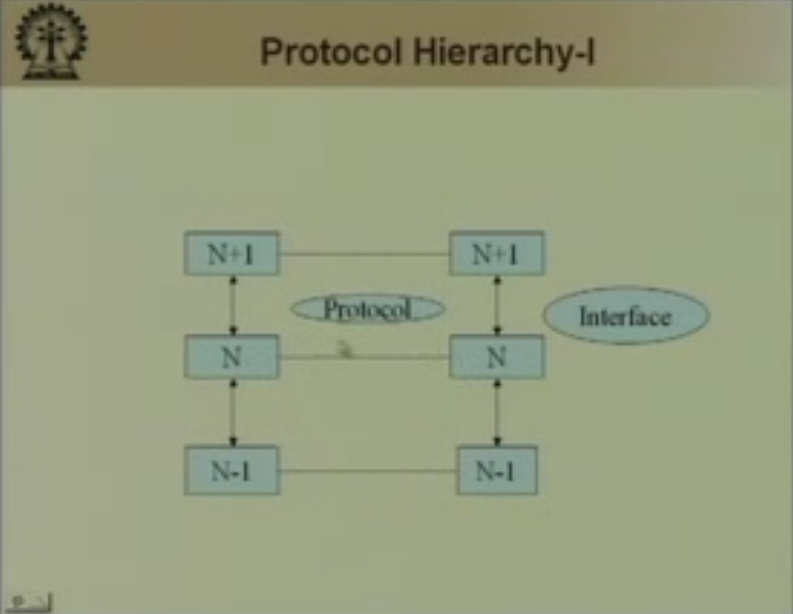
\includegraphics[scale=0.5]{Selection_001}
\end{center}
\begin{itemize}
\item Most networks are organised as series of layers
\item The task of each layer is to  provide service to its upper layer 
\item Every layer is virtually connected to its peer.
\pagebreak
\item There is a peer to peer protocol running between any two corresponding and communicating layers.
\item The interface between the layers in the same node is well defined.
\item The implementation of each layer in each node is transparent to other layers.
\item The peer to peer layer protocols can be changed if the peers all agree. However it need not be referred to other layers.
\item The service definition tells what the layer does and nothing else.
\item The interface tells the process above how to access it, what the parameters are and what are the results to expect.
\item Known protocol stacks are:
\begin{itemize}
\item OSI reference model
\item TCP/IP reference model
\item ATM reference model
\item There are some other protocol stacks as well and some new ones too.
\end{itemize}
\end{itemize}

\section{OSI Reference Model}
\begin{enumerate}
\item Application Layer
\item Presentation Layer
\item Session Layer
\item Transport Layer
\item Network Layer
\item Data link layer
\item Physical Layer
\end{enumerate}

\section{Peer Level Communication}
\begin{itemize}
\item Message sent from one application to another on different layers.
\begin{itemize}
\item travels down the layers of the sending machine as each layer adds up its header to the message.
\item bottom-most layer (physical layer) sends the message to the receiving machine.
\end{itemize}
\item Sending message
\begin{itemize}
\item Received by physical layer on the other side.
\item Passed up through each layer.
\item 
\end{itemize}
\end{itemize}

\section{OSI Model: 7 protocol layers}
\begin{itemize}
\item \textbf{Physical} - How to transmit bits.
\item \textbf{Data Link} - How to transmit frames.
\item \textbf{Network} - How to route packets to the node.
\item \textbf{Transport} - How to send packets to the application.
\item \textbf{Session} - Manage connections
\item \textbf{Presentation} - Encode/Decode messages, Security
\item \textbf{Application} - Everything else!
\end{itemize}

\section{Application Layer}
\begin{itemize}
\item The application layer contains a variety of protocols which are used by various applications e.g smtp, ftp, http etc.
\item The application layer usually contains some cheap connection to its peers. Example of peers are nodes giving some service and its clients.
\end{itemize}

\section{Presentation Layer}
\begin{itemize}
\item Handles the format of the data.
\begin{itemize}
\item Protocol conversion
\item Data translation (ASCII)
\item Compression
\item Encryption
\end{itemize}
\end{itemize}

\section{Session Layer}
\begin{itemize}
\item Allows application on different layers to share a connection.
\item Provides checkpoints, if a connection is lost only the required info is resent.
\item Dialog control who can transmit.
\end{itemize}

\section{Transport Layer}
The basic functionality of transport layer is to accept data from layer above, split it into smaller units if necessary and ensure that the pieces all arrive at the right order at the other end. This should also be done in a cheap and efficient manner and isolate the upper layers from change in technology.
\\[0.5cm]
\textbf{Types of transport services:}
\begin{itemize}
\item Error free point to point channel that delivers message or bytes in the order in which they were sent.
\item Transport of isolated messages with no guarantee of delivery.
\item Broadcasting of messages to multiple destinations.
\end{itemize}

\section{Network Layer}
\begin{itemize}
\item It decides on what route to take locally so that intended message ultimately reaches its destination.
\item It controls broadcasting by essentially segregating multiple networks.
\item It handles technological mismatches like restriction on packet sizes.
\item Congestion control is done in this layer.
\item Billing information may be generated in this layer.
\item It handles different policies pertaining to different networks.
\item In broadcast networks, its functionality is minimal. 
\end{itemize}

\section{Data link Layer}
\begin{itemize}
\item Make physical layer appear like it is free of transmission errors.
\item Handle rate mismatch between sender and receiver.
\item Control access of channels which are broadcast in nature.
\end{itemize}

\section{Physical Layer}
\begin{itemize}
\item This transmits raw bits over a communication channel.
\item Physical issues like voltages, attenuation and noise levels, light intensity, ports and pins, modulating techniques are described in this level.
\end{itemize}
\begin{center}
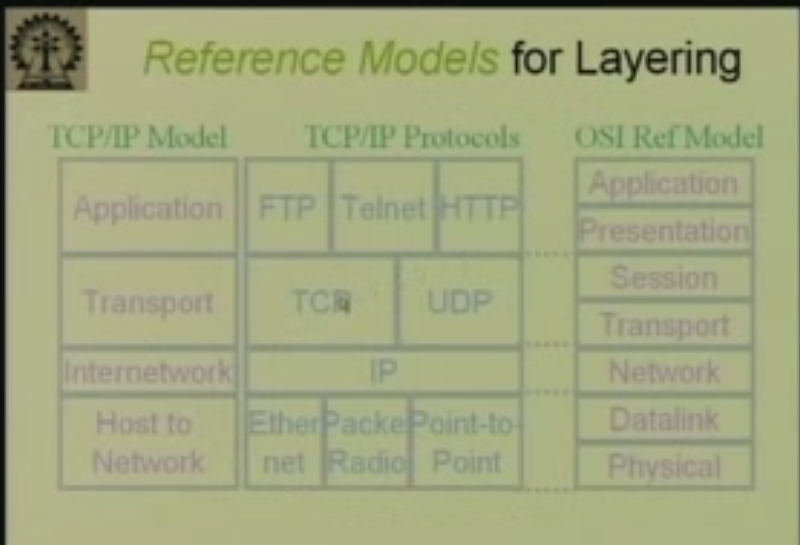
\includegraphics[scale=0.3]{Selection_002.png}
\end{center}
\end{document}